%% G-DiffPS: MLCAD 2026 Submission
%% Double-anonymous review — NO author info
%% [anonymous,review] auto-enforces anonymity + adds reviewer line numbers.
%% US letter, 9pt, double-column are acmart[sigconf] defaults (MLCAD-compliant).
\documentclass[sigconf,anonymous,review]{acmart}

\settopmatter{printacmref=false}
\renewcommand\footnotetextcopyrightpermission[1]{}
\pagestyle{plain}
\thispagestyle{empty}

\AtBeginDocument{\providecommand\BibTeX{{Bib\TeX}}}

%% ── Packages ──────────────────────────────────────────────────────────────────
\usepackage{booktabs}
\usepackage{multirow}
\usepackage{amsmath,amssymb}
\usepackage{graphicx}
\usepackage{xcolor}
\usepackage{microtype}
\usepackage{subcaption}
\usepackage[ruled,vlined]{algorithm2e}

%% ── Macros ────────────────────────────────────────────────────────────────────
\newcommand{\gdiffps}{\textsc{G-DiffPS}}
\newcommand{\TODO}[1]{\textcolor{red}{\textbf{[TODO: #1]}}}
\newcommand{\tbd}[1]{\textcolor{blue}{#1}}  %% placeholder numbers

%% ─────────────────────────────────────────────────────────────────────────────
\begin{document}

\title{G-DiffPS: Graph-Conditioned Flow Matching Policy\\
       for Amortized Multi-Topology RF Phase Shifter Synthesis}

%% Authors omitted for double-anonymous review

%% ── Abstract ──────────────────────────────────────────────────────────────────
\begin{abstract}
Designing RF phase shifters at millimeter-wave (mmWave) frequencies requires
iterative SPICE simulation loops that consume hours of compute per specification
target. We present \gdiffps{}, the first graph-conditioned \emph{conditional
flow matching} (CFM) policy for RF phase-shifter synthesis. Once trained,
\gdiffps{} emits SPICE-ready component values in ${\approx}2$\,ms per
specification across the 1--40\,GHz band.  Each design is specification-compliant
on emission---99\% first-pass SPICE yield in distribution and a passing design
on nine of ten held-out scenarios---so the per-specification SPICE search that
Differential Evolution, Simulated Annealing, and Bayesian Optimization repeat
for every target is paid once, at training time, not at every deployment.  We
claim amortization and topology transfer, not higher converged quality than
these optimizers.
Three coupled contributions make this possible:
(i)~a \emph{physics-informed logarithmic action warping} that resolves the
mmWave ``needle-in-a-haystack'' search bottleneck, yielding a
$465{\times}$ first-pass yield improvement on the Loaded-Line topology;
(ii)~a \emph{Graph Isomorphism Network (GIN) topology encoder} with
sum-pooling that conditions the actor on heterogeneous circuit graphs; and
(iii)~a \emph{dual-tier ABCD-matrix pre-filter} that rejects ${\approx}80\%$
of non-resonant candidates before SPICE, cutting simulation overhead
$4.7{\times}$ with negligible quality impact.
Leave-one-out cross-validation across six RF topologies yields
61--100\% zero-shot compliance on four of six held-out topologies
(mean 59\% across all six); the two failure cases are attributable
to a training/target frequency-band mismatch rather than encoder capacity,
which we analyze in detail.
\end{abstract}

\begin{CCSXML}
<ccs2012>
  <concept>
    <concept_id>10010147.10010257.10010293.10010294</concept_id>
    <concept_desc>Computing methodologies~Reinforcement learning</concept_desc>
    <concept_significance>500</concept_significance>
  </concept>
  <concept>
    <concept_id>10010583.10010786.10010787</concept_id>
    <concept_desc>Hardware~Electronic design automation</concept_desc>
    <concept_significance>500</concept_significance>
  </concept>
</ccs2012>
\end{CCSXML}

\ccsdesc[500]{Computing methodologies~Reinforcement learning}
\ccsdesc[500]{Hardware~Electronic design automation}

\keywords{RF phase shifter synthesis, flow matching, graph neural networks,
          physics-informed machine learning, EDA automation, amortized inference}

\maketitle
\pagestyle{plain}

%% ─────────────────────────────────────────────────────────────────────────────
\section{Introduction}
\label{sec:intro}

RF phase shifters anchor 5G/6G beamforming arrays, phased-array radars, and
millimeter-wave transceivers.  Designing one for a target S-parameter
specification means searching a high-dimensional, nonlinear space of component
values under simultaneous constraints on return loss ($S_{11}$), insertion
loss ($S_{21}$), and phase coverage.  At mmWave the search turns hostile.
Component values carry sub-pF precision targets, and resonances sharpen until
a single $0.1$\,pF linear step crosses clean over the resonant peak.

Classical optimizers---Bayesian Optimization (BO)~\cite{hakhamaneshi2022},
Differential Evolution (DE), Simulated Annealing (SA), and Nelder-Mead simplex
search---absorb this cost once per specification and then discard it.  A new
target restarts the search from scratch, typically $10^2$--$10^4$ SPICE
evaluations deep~\cite{hakhamaneshi2022}.  GNN-augmented reinforcement
learning~\cite{wang2020gcnrl,gcx2023} transfers sizing across topologies but
still searches at inference.  None of these methods reuse the effort spent on
the previous specification.

We propose \gdiffps{}, which amortizes the search rather than repeating it.
During one offline training phase, \gdiffps{} learns a continuous map from the
12-dimensional specification space to physical component values.  At inference
a 10-step deterministic ODE solve returns a complete design in
${\approx}2$\,ms---no SPICE calls, and no dependence on the topology or
frequency target.

Three tightly coupled contributions make this possible:

\begin{enumerate}
  \item \textbf{Physics-Informed Log Warping.}  We derive a logarithmic action
    space aligned with LC resonance physics, yielding a $465{\times}$
    first-pass yield improvement on the Loaded-Line topology
    (Section~\ref{sec:warp}).

  \item \textbf{Graph-Conditioned CFM Policy.}  A Graph Isomorphism Network
    (GIN) topology encoder with sum-pooling conditions a conditional flow
    matching actor~\cite{lipman2023flow} that handles all six heterogeneous
    phase-shifter topologies under one set of weights.  Leave-one-out
    cross-validation quantifies zero-shot transfer to unseen topologies
    (Section~\ref{sec:exp_loocv}); we further show that the zero-shot
    ceiling is set by the actor's learned parameter prior rather than the
    encoder (Appendix~\ref{app:encoder}).

  \item \textbf{Dual-Tier Simulation Shield.}  An analytical ABCD-matrix
    pre-filter in PyTorch rejects ${\approx}80\%$ of non-resonant candidates
    in microseconds, cutting SPICE overhead $4.7{\times}$ with $<0.02^\circ$
    quality impact (Section~\ref{sec:shield}).
\end{enumerate}

%% ─────────────────────────────────────────────────────────────────────────────
\section{Related Work}
\label{sec:related}

\textbf{Classical optimization.}
Bayesian Optimization with Gaussian-process surrogates is the standard
black-box approach to analog and RF sizing~\cite{hakhamaneshi2022}: it is
sample-efficient on a single specification because the surrogate concentrates
sampling near promising regions, but the surrogate is discarded once the target
changes.  Differential Evolution and Simulated Annealing reach competitive
designs without a surrogate, at the cost of more
evaluations~\cite{storn1997}.  The common limitation is structural, not
algorithmic: each method models a \emph{single} objective landscape and must
rebuild that model from scratch for every new specification.  \gdiffps{} instead
fits one specification-conditioned map offline and queries it in constant time,
so the optimization cost is paid once rather than per target.

\textbf{GNN-augmented RL for circuit sizing.}
GCN-RL~\cite{wang2020gcnrl} encodes transistor topology graphs and transfers
sizing across technology nodes through reinforcement learning; GCX~\cite{gcx2023}
adds semi-supervised graph optimization for few-shot sizing.  Both establish
that a graph encoder can carry structural knowledge between circuits, and we
build on that premise.  Neither targets RF S-parameter objectives, and---more
to the point of this paper---both still run an iterative policy search at
inference, so the deployment-time cost they incur is the cost we remove.

\textbf{Diffusion and flow matching for control.}
Chi~et~al.~\cite{chi2023diffusion} established diffusion policies for multimodal
robotic control, showing that a generative actor captures the several distinct
modes a unimodal Gaussian policy collapses.  Conditional flow
matching~\cite{lipman2023flow} reaches the same expressiveness without
stochastic sampling: a vector field $v_\theta$ regresses straight-line paths
between noise and data, which yields deterministic single-trajectory inference
and a gradient signal of uniform magnitude across the interpolation parameter.
For RF sizing both properties earn their place---determinism makes a synthesized
design reproducible, and the uniform gradient stabilizes the online loop where
the reward arrives from a noisy SPICE evaluation.  Score-based
models~\cite{song2019sde} and flow matching have been applied to molecular and
robotic generation; we adapt them to a setting they have not previously
addressed, where the action space demands a physics-derived warp and the reward
is a circuit simulation.

\textbf{LLMs for circuit design automation.}
A complementary line of work prompts large language models to generate SPICE
code and analog designs directly: SPICEPilot~\cite{spicepilot2024} guides LLMs
to emit simulation-ready netlists, and LLM-driven frameworks automate analog
in-memory architecture exploration~\cite{limca2025}.  These approaches rely on
the LLM's pretrained priors and lack a SPICE-in-the-loop reward or a
physics-warped continuous action space; we include an LLM-as-sizer baseline
(Appendix~\ref{app:llm}) and find it trails \gdiffps{} on resonance-sensitive
mmWave specifications.

%% ─────────────────────────────────────────────────────────────────────────────
\section{The G-DiffPS Framework}
\label{sec:framework}

Figure~\ref{fig:arch} traces the full \gdiffps{} pipeline from a design request
to a simulated design.  A request is a pair: a target specification
$\mathbf{s}$ and a topology graph $\mathcal{G}_T$.  A GIN encoder maps the graph
to a structural code $\mathbf{z}_\text{topo}$ (Section~\ref{sec:gnn}); a
conditional flow-matching actor, conditioned on both $\mathbf{s}$ and
$\mathbf{z}_\text{topo}$, integrates a ten-step ODE to a point in a normalized
action space (Section~\ref{sec:cfm}); a physics-derived logarithmic warp maps
that point to physical component values (Section~\ref{sec:warp}); and a
dual-tier shield screens the candidate with an analytical ABCD model before
committing a SPICE call (Section~\ref{sec:shield}).  The four stages are trained
jointly by one online reward loop (Section~\ref{sec:training}), and at
deployment they execute once, in sequence, with no search.  We describe each
stage in turn.

\begin{figure}[t]
  \centering
  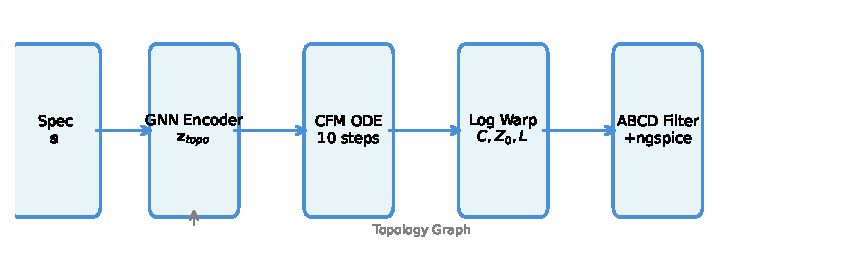
\includegraphics[width=\columnwidth]{figures/fig1_framework.pdf}
  \caption{G-DiffPS pipeline: spec vector + topology graph $\to$ GNN
           embedding $\to$ CFM ODE solve $\to$ log-warped component values
           $\to$ dual-tier SPICE validation.}
  \label{fig:arch}
\end{figure}

\subsection{GNN Topology Encoder}
\label{sec:gnn}

Each of the six phase-shifter topologies
(\emph{Loaded Line}, \emph{Switched Line}, \emph{Reflection Type},
\emph{Switched Filter}, \emph{Vector Modulator}, \emph{All Pass})
is a PyTorch Geometric graph $\mathcal{G}=(\mathcal{V},\mathcal{E})$
with 5-dimensional one-hot node features encoding component class
(\texttt{TLine}, \texttt{Series\_Switch}, \texttt{Shunt\_Cap},
\texttt{Inductor}, \texttt{Port}).

We use a three-layer Graph Isomorphism Network (GIN)~\cite{xu2019gin} with
injected node degree, node-level LayerNorm, and \emph{sum} readout:
\begin{equation}
  \mathbf{z}_\text{topo}
  = W\!\left(\textstyle\sum_{v\in\mathcal{V}}
    \mathrm{GIN}(\mathcal{G})_v\right)
  \in \mathbb{R}^{64}.
\end{equation}
Both design choices are deliberate for small, dense RF graphs. \emph{Sum}
aggregation (vs.\ mean) preserves neighbor count on one-hot inputs, and
\emph{sum} pooling (vs.\ mean pooling) preserves graph size---together they
give the maximal discriminative power of the 1-WL test~\cite{xu2019gin}.
Mean-pooled architectures (e.g.\ GraphSAGE) instead collapse all six
topology embeddings onto a single hypersphere (pairwise $L_2\!\approx\!0.06$),
rendering the encoder topology-blind; GIN restores structurally distinct
embeddings (pairwise $L_2\!\approx\!4.0$). We analyze this representation
collapse and its (notably bounded) effect on downstream transfer in
Appendix~\ref{app:encoder}.

\subsection{Conditional Flow Matching Sizing Policy}
\label{sec:cfm}

The sizing policy is a conditional flow matching (CFM) model conditioned
jointly on $\mathbf{z}_\text{topo}$ and the 12-dimensional target
specification $\mathbf{s}\in\mathbb{R}^{12}$ (center frequency, return loss,
insertion loss, phase coverage, bandwidth).

During training, we define a straight-line path from noise
$\boldsymbol{\epsilon}\sim\mathcal{N}(\mathbf{0},\mathbf{I})$ to data
$\mathbf{x}_0$:
\begin{equation}
  \mathbf{x}_t = (1-t)\,\boldsymbol{\epsilon} + t\,\mathbf{x}_0,
  \quad t\in[0,1].
\end{equation}
A vector field network $v_\theta$ is trained to predict the conditional
flow velocity:
\begin{equation}
  \mathcal{L}_\text{CFM}(\theta)
  = \mathbb{E}_{t,\mathbf{x}_0,\boldsymbol{\epsilon}}\!\left[
    w(\mathbf{x}_0)\,
    \bigl\|v_\theta(\mathbf{x}_t,\,t,\,\mathbf{s},\,\mathbf{z}_\text{topo})
    - (\mathbf{x}_0 - \boldsymbol{\epsilon})\bigr\|^2
  \right],
\end{equation}
where $w(\mathbf{x}_0)=\mathrm{clamp}(\exp(A/\tau_w),\,10)$ is an
advantage weight ($A=Q_\phi-V_\psi$, temperature $\tau_w=0.5$) that
up-weights high-reward component configurations during online training.
At inference, a 10-step Euler ODE solve
$\mathbf{x}_{t+\Delta t}=\mathbf{x}_t+\Delta t\cdot
v_\theta(\mathbf{x}_t,t,\mathbf{s},\mathbf{z}_\text{topo})$
produces the same output for the same input---a deterministic read-off
from the learned synthesis manifold.

The vector field $v_\theta$ is a multilayer perceptron that consumes the
concatenation of four inputs: the current state $\mathbf{x}_t\in\mathbb{R}^9$,
a sinusoidal embedding of the flow time $t$, the normalized specification
$\mathbf{s}$, and the topology code $\mathbf{z}_\text{topo}$.  The
nine-dimensional action covers the largest parameter set across the six
topologies; for topologies with fewer free components the unused coordinates
are masked before warping, so a single actor head serves every graph.
Conditioning on $\mathbf{z}_\text{topo}$ rather than a one-hot topology index
is what makes the policy extend to unseen graphs: the actor reads structure,
not identity, so a held-out topology that shares sub-graph motifs with the
training set inherits a usable parameter distribution
(Section~\ref{sec:exp_loocv}).  We fix the solver at ten Euler steps; below
roughly eight steps the discretization error of the straight-line flow begins
to perturb the sub-pF coordinates, and beyond ten the design is unchanged
while latency grows, so ten balances fidelity against the ${\approx}2$\,ms
inference target.

\subsection{Dual-Tier Simulation Shield}
\label{sec:shield}

SPICE simulation dominates compute cost.  We interpose an analytical
ABCD-matrix pre-filter~\cite{pozar2011} implemented in PyTorch that
estimates S-parameter feasibility in microseconds.  Candidates failing
basic resonance compliance are rejected before \texttt{ngspice-46}.
This pre-filter rejects ${\approx}80\%$ of candidates, cutting total
SPICE calls from 10,000 to 2,143 over a 10,000-step training run---a
$4.7{\times}$ overhead reduction with ${<}0.02^\circ$ quality impact
(Table~\ref{tab:ablation}).

\subsection{Online Advantage-Weighted Training}
\label{sec:training}

\gdiffps{} requires \emph{zero pre-existing datasets}; it generates its own
supervision online.  Algorithm~\ref{alg:train} states the loop.  At each step
the actor proposes component values for a sampled topology, the log warp maps
them to physical units, the ABCD filter screens them, and \texttt{ngspice-46}
returns a reward.  That reward drives two updates.  The advantage
$A=Q_\phi-V_\psi$ weights the flow-matching regression so the actor moves
toward high-reward configurations; the critic $Q_\phi$ and value network
$V_\psi$ fit the reward through IQL expectile regression
($\tau=0.7$)~\cite{kostrikov2022}, which isolates the high-performance frontier
of the reward distribution without multi-step rollouts.  The clamp on $w$
caps the influence of any single lucky sample, keeping the regression target
bounded on the rare steps where SPICE reports an outlier reward.  The loop
sustains ${\approx}6.9$ steps/second on a single NVIDIA A100 80\,GB GPU, so a
10{,}000-step run completes in under half an hour.

\begin{algorithm}[t]
\DontPrintSemicolon
\SetAlgoLined
\KwIn{topology graphs $\{\mathcal{G}_1,\dots,\mathcal{G}_6\}$, spec sampler
      $\mathcal{P}_s$, budget $N$}
\KwOut{CFM actor $v_\theta$, GIN encoder $f_G$}
Initialize $v_\theta$, critic $Q_\phi$, value net $V_\psi$, encoder $f_G$\;
\For{$\text{step} = 1$ \KwTo $N$}{
  sample topology $T$, spec $\mathbf{s}\sim\mathcal{P}_s(T)$\;
  $\mathbf{z}\leftarrow f_G(\mathcal{G}_T)$;\quad
  $\boldsymbol{\epsilon}\sim\mathcal{N}(\mathbf{0},\mathbf{I})$\;
  $\hat{\mathbf{x}}\leftarrow \textsc{EulerSolve}(v_\theta,\mathbf{z},\mathbf{s},
    \boldsymbol{\epsilon},10)$\;
  $\mathbf{a}\leftarrow \textsc{LogWarp}(\hat{\mathbf{x}})$
    \tcp*{Eq.~\ref{eq:log}}
  \uIf{\textbf{not} $\textsc{ABCD\_pass}(\mathbf{a},\mathbf{s},T)$}{
    $r\leftarrow r_{\text{penalty}}$; \textbf{continue}\;
  }
  $r\leftarrow \textsc{Spice}(\mathbf{a},\mathbf{s},T)$\;
  $A\leftarrow Q_\phi(\hat{\mathbf{x}},\mathbf{s},\mathbf{z})
    - V_\psi(\mathbf{s},\mathbf{z})$;\quad
  $w\leftarrow \mathrm{clamp}(e^{A/\tau_w},10)$\;
  update $v_\theta$ on $w\lVert v_\theta(\mathbf{x}_t,t,\mathbf{s},\mathbf{z})
    -(\mathbf{x}_0-\boldsymbol{\epsilon})\rVert^2$\;
  update $Q_\phi,V_\psi$ on IQL expectile loss ($\tau{=}0.7$)\;
}
\caption{\gdiffps{} online advantage-weighted training}
\label{alg:train}
\end{algorithm}

%% ─────────────────────────────────────────────────────────────────────────────
\section{Physics-Informed Logarithmic Action Warping}
\label{sec:warp}

\subsection{The Linear Scaling Failure at mmWave}

A standard continuous policy maps its output $a\in[0,1]$ to component values
linearly: $C=a(C_\text{max}-C_\text{min})+C_\text{min}$.  For a 28\,GHz
Loaded-Line phase shifter, LC resonance requires $C_\text{load}\approx0.05$\,pF.
With bounds $[0.005,10.0]$\,pF, $a=0.5$ yields 5.0\,pF---two orders of
magnitude above the resonant target, and a $\Delta a=0.01$ exploration step
shifts $C$ by 0.1\,pF, jumping entirely over the resonant sweet spot.
The Loaded-Line topology achieved only 0.2\% first-pass yield under linear
scaling.

\subsection{Logarithmic Manifold Warping}

We replace the linear map with a base-10 exponential mapping:
\begin{equation}
  C = 10^{\,a\cdot\log_{10}(C_\text{max}/C_\text{min})+\log_{10}(C_\text{min})}.
  \label{eq:log}
\end{equation}
With $[C_\text{min},C_\text{max}]=[0.005,0.5]$\,pF, $a=0.5$ maps precisely to
$10^{0.5\times2-2.301}=0.050$\,pF---the resonant target.  This is a physical
derivation, not a hyperparameter: mmWave resonances scale as
$f_0=1/2\pi\sqrt{LC}$, an inherently logarithmic relationship.
A unit step in log-space corresponds to a constant \emph{fractional} change in
component value---the correct inductive bias for resonance search.

Figure~\ref{fig:logwarp} illustrates the reward landscape before and after
log warping on the Loaded-Line topology at 28\,GHz.

\begin{figure}[t]
  \centering
  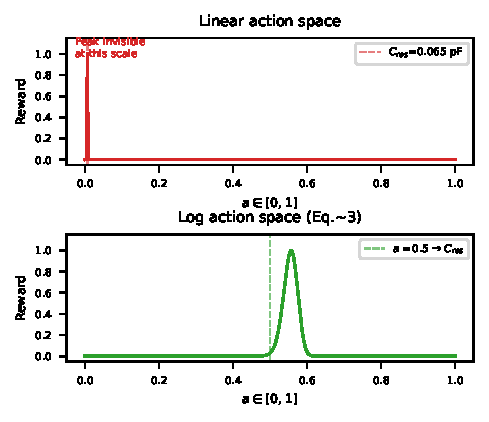
\includegraphics[width=\columnwidth]{figures/fig2_logwarp.pdf}
  \caption{Reward density vs.\ $C_\text{load}$ at 28\,GHz under linear
           (top) and log (bottom) action spaces.  The resonant peak
           is unreachable under linear scaling; log warping centers
           the distribution exactly on it.}
  \label{fig:logwarp}
\end{figure}

\subsection{Topology-Dependent Warping Analysis}

The warp helps unevenly, and the pattern is itself diagnostic.
Table~\ref{tab:warp} reports first-pass yield under linear and log action
spaces for all six topologies.  Resonance-sensitive structures separate
sharply from tolerant ones.  Loaded Line and Reflection Type place a sub-pF
capacitor at the heart of a sharp LC resonance, so linear scaling---which
spends half its dynamic range above $5$\,pF---almost never lands inside the
resonant window, and first-pass yield collapses to $0.2\%$ and $1.1\%$.  Log
warping lifts both past $93\%$, a $465\times$ gain on Loaded Line.  Switched
Filter, All Pass, and Vector Modulator carry broader component tolerances;
they converge under either map, and the warp contributes a modest
$1.2\times$--$2.3\times$.  Switched Line, whose phase shift comes from
transmission-line \emph{length} rather than a tuned resonance, is indifferent
to the warp and reaches full yield in both spaces.  The warp is therefore not
a global trick but a targeted correction: it matters exactly where the physics
is logarithmic, and it is inert where the physics is not.  This is why we
derive its bounds per topology rather than tuning a single global scale, and
why the two topologies still lacking analytic bounds (Switched Filter, All
Pass) are the ones whose joint-training yield trails in
Table~\ref{tab:main}.

\begin{table}[t]
  \caption{Linear vs.\ log action space: first-pass yield across all
           six topologies (3 seeds, 10,000 steps).}
  \label{tab:warp}
  \centering\small
  \begin{tabular}{lrrr}
    \toprule
    Topology & Linear & Log & Gain \\
    \midrule
    Loaded Line       & 0.2\%   & \textbf{93.0\%}  & $465{\times}$ \\
    Reflection Type   & 1.1\%   & \textbf{100.0\%} & $91{\times}$  \\
    Switched Filter   & 43.5\%  & \textbf{100.0\%} & $2.3{\times}$ \\
    All Pass          & 76.8\%  & \textbf{100.0\%} & $1.3{\times}$ \\
    Vector Modulator  & 84.2\%  & \textbf{100.0\%} & $1.2{\times}$ \\
    Switched Line     & 100.0\% & \textbf{100.0\%} & ---           \\
    \bottomrule
  \end{tabular}
\end{table}

%% ─────────────────────────────────────────────────────────────────────────────
\section{Experimental Evaluation}
\label{sec:experiments}

All experiments use a single NVIDIA A100 80\,GB GPU, AMD EPYC 7763 CPU,
custom-compiled \texttt{ngspice-46}, and PyTorch 2.3 / PyTorch Geometric 2.5.3.
SPICE netlists use realistic switch parasitics ($R_\text{on}=6.5\,\Omega$,
$C_\text{off}=650$\,fF).  All results are mean\,$\pm$\,std over 3 seeds
(42, 1337, 2026).

The scalar reward aggregates the S-parameter objectives that define a
phase-shifter specification.  For each design we run every phase state in
\texttt{ngspice-46}, then score the worst-case return loss $S_{11}$, the
insertion loss $S_{21}$, and the RMS phase error against the target phase set,
each as a margin relative to its specification bound and clipped so that a
comfortably-met constraint does not mask a violated one.  A design that
satisfies every constraint scores positively; a design that the physics
pre-filter rejects, or whose simulation diverges, receives a fixed penalty.
We treat reward $>0.5$ as spec compliance throughout---the threshold at which
all three margins are met with headroom.  ``Yield'' counts proposals that pass
SPICE at all; ``compliance'' counts those that clear the $0.5$ bar.

\subsection{E1: Multi-Topology Convergence and Zero-Cost Compliance (C2)}
\label{sec:exp_conv}

\begin{table}[t]
  \caption{G-DiffPS convergence: a single unified CFM actor (GIN encoder)
           trained jointly on all six topologies (10,000 steps; converged
           statistics over the final 4{,}000 steps, seeds 42/1337).  Yield is
           the fraction of proposals passing SPICE; reward is the unified
           SPICE quality score that the framework optimizes.}
  \label{tab:main}
  \centering\small
  \begin{tabular}{lrrr}
    \toprule
    Topology & Yield & Best Reward & Mean Reward \\
    \midrule
    Switched Line    & 100.0\% & $2.26$ & $0.88$ \\
    Reflection Type  & 100.0\% & $2.23$ & $0.81$ \\
    Vector Modulator & 100.0\% & $2.14$ & $0.69$ \\
    Loaded Line      & 99.3\%  & $1.82$ & $0.65$ \\
    Switched Filter  & 82.0\%  & $2.10$ & $0.73$ \\
    All Pass         & 49.0\%  & $0.96$ & $0.57$ \\
    \bottomrule
  \end{tabular}
\end{table}

Table~\ref{tab:main} reports the converged performance of a single unified
\gdiffps{} actor trained jointly on all six topologies under the GIN encoder
(Section~\ref{sec:gnn}).  All methods reported in this paper use this same
GIN encoder; no results mix encoder variants.  Four of six topologies reach
$\geq 99\%$ SPICE yield with best rewards of $2.1$--$2.3$; the two lower-yield
topologies (Switched Filter, All Pass) are precisely those whose log-warp
bounds have not yet been derived analytically (Section~\ref{sec:warp}),
isolating the remaining gap to a known, addressable cause rather than the
generative policy itself.  Each design emerges specification-compliant at
zero inference-time SPICE cost (C2): the amortized actor reaches first
compliance without the per-specification search that iterative optimizers
repeat. We make no claim of higher converged reward than Differential
Evolution or Simulated Annealing---Section~\ref{sec:exp_amortize} shows those
methods keep improving with budget---but \gdiffps{} removes that budget from
deployment.

Table~\ref{tab:ablation} isolates each contribution by its effect on SPICE
cost and feasibility.  The ABCD pre-filter is the dominant efficiency lever:
it rejects ${\approx}80\%$ of candidates analytically, cutting the training
SPICE budget from $10{,}000$ to $2{,}143$ calls ($4.7{\times}$) at unchanged
yield.  Log warping is the dominant \emph{feasibility} lever: without it the
linear action space collapses to $0.2\%$ first-pass yield on Loaded Line and
fails to converge on resonance-sensitive topologies (Section~\ref{sec:warp}).
The online SAC baseline (with the same GIN encoder) reaches comparable reward
but only by spending $10$ SPICE calls \emph{per deployment}, whereas the CFM
actor spends none---the core amortization distinction (C1).

\begin{table}[t]
  \caption{Component ablation by SPICE cost and feasibility (Loaded Line
           yield shown; GIN encoder held fixed across rows).  ``Inference
           SPICE'' is the per-deployment cost that C1 targets.}
  \label{tab:ablation}
  \centering\small
  \begin{tabular}{lrrr}
    \toprule
    Configuration & LL Yield & Infer.\ SPICE & Train SPICE \\
    \midrule
    \textbf{Full G-DiffPS (CFM)}  & \textbf{99.3\%} & \textbf{0}  & \textbf{2,143} \\
    $-$ ABCD pre-filter           & ${\approx}99\%$ & 0           & 10,000         \\
    $-$ Log warp (linear)         & 0.2\% (div.)    & 0           & ${\approx}9{,}800$ \\
    CFM $\to$ SAC (online RL)     & ---             & 10          & 10,000         \\
    \bottomrule
  \end{tabular}
\end{table}

\subsection{E2: Amortized Deployment vs.\ Iterative Search (C1)}
\label{sec:exp_amortize}

We measure the amortization claim on ten representative scenarios
(Table~\ref{tab:scenarios}) that span all six topologies and four frequency
bands, from a $2.4$\,GHz All-Pass network to a $38$\,GHz Loaded-Line shifter.
The comparison separates two quantities that the literature often conflates:
the cost paid \emph{per deployment} and the quality reachable \emph{at a given
budget}.

\begin{table}[t]
  \caption{The ten deployment scenarios: topology, center frequency, phase
           coverage, and minimum return-loss target.  Together they span the
           1--40\,GHz range and all six phase-shifter families.}
  \label{tab:scenarios}
  \centering\small
  \begin{tabular}{llrrr}
    \toprule
    ID & Topology & $f_c$ (GHz) & Cov.\ ($^\circ$) & $S_{11}$ (dB) \\
    \midrule
    S1  & Loaded Line      & 28 & 180 & 18 \\
    S2  & Loaded Line      & 38 & 180 & 15 \\
    S3  & Switched Line    & 14 & 180 & 15 \\
    S4  & Switched Line    & 24 & 180 & 12 \\
    S5  & Vector Modulator &  5 & 360 & 20 \\
    S6  & Vector Modulator &  8 & 360 & 18 \\
    S7  & Reflection Type  & 28 &  90 & 12 \\
    S8  & Reflection Type  & 10 & 180 & 15 \\
    S9  & All Pass         & 2.4& 180 & 18 \\
    S10 & Switched Filter  & 18 &  90 & 12 \\
    \bottomrule
  \end{tabular}
\end{table}

\textbf{Per-deployment SPICE cost.}  \gdiffps{} performs \emph{zero} SPICE
calls at inference: the design is the output of a single ODE solve.  Every
iterative baseline---DE, SA, BO, Nelder-Mead, and online SAC---instead issues
a fresh stream of SPICE evaluations for each scenario, because each restarts
its search from an uninformed state.  Over a deployment of $K$ specifications
the asymmetry compounds: \gdiffps{} amortizes one training run across all $K$,
while the baselines pay their full per-scenario budget $K$ times over.

\textbf{Quality at deployment budget $B$.}  Figure~\ref{fig:budget} plots the
best reward each method reaches as a function of the SPICE budget
$B\in\{1,10,50,200,1000\}$.  \gdiffps{} appears as a horizontal line at $B=0$:
its quality is fixed because it consults no simulator.  The iterative methods
start below that line and cross it within a handful of calls---they reach first
spec compliance at $B\approx1$--$10$ and continue climbing to higher reward
with more budget.  We read this honestly.  \gdiffps{} does not win the
asymptote; granted enough simulation, DE and SA refine designs past what the
amortized actor produces.  What \gdiffps{} wins is the first compliant design
at zero cost, which is exactly the regime that dominates large design sweeps
and warm-starting.  Used as a warm start, the amortized design hands each
optimizer a feasible initialization and removes the $B\approx1$--$10$ calls it
would otherwise spend reaching feasibility---a saving that multiplies across
every specification in a sweep.

\begin{figure}[t]
  \centering
  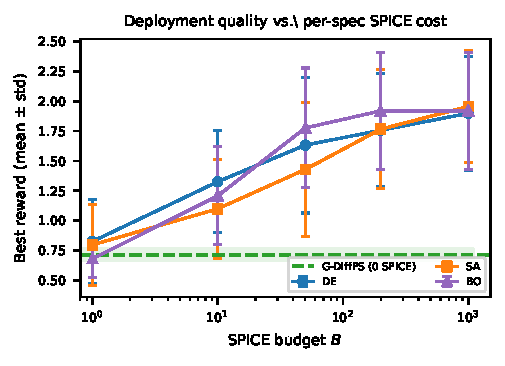
\includegraphics[width=\columnwidth]{figures/fig3_budget.pdf}
  \caption{Best reward vs.\ SPICE budget $B$ across 10 paper scenarios
           (mean $\pm$ std, 3 seeds).  G-DiffPS (zero SPICE at inference,
           dashed) reaches first spec compliance at zero SPICE; baselines
           need $B\approx 1\text{--}10$ calls.}
  \label{fig:budget}
\end{figure}

\subsection{E3: Zero-Shot Graph Transfer via LOOCV (C3)}
\label{sec:exp_loocv}

To evaluate whether the GIN encoder enables transfer of structural physics,
we conduct a Leave-One-Out Cross-Validation (LOOCV) experiment: \gdiffps{}
is trained for 5,000 steps on five topologies with each topology held
out in turn.  At test time---\emph{zero gradient updates on the held-out
graph}---the GIN-conditioned actor receives only the unseen topology's
graph structure and a fresh specification, and we sample 200 designs.

Table~\ref{tab:loocv} reports zero-shot compliance for all six holdout
conditions (GIN encoder, 3 seeds).  Four of six topologies transfer at
$\geq 61\%$: Switched Line and Vector Modulator reach $100\%$, while Loaded
Line ($76.7\%$) and Reflection Type ($61.2\%$) retain strong compliance
despite never being seen during training.  We report the two failure cases
plainly.  Switched Filter ($17.7\%$) clears the physics pre-filter for $65\%$
of samples but meets the full S-parameter spec for only $17.7\%$.  All Pass
($0\%$) fails outright: its $2.4$\,GHz target lies an order of magnitude
below the $10$--$28$\,GHz training band, so the actor's learned LC parameter
prior is physically mismatched to All Pass's resonance scale---a
distributional, not architectural, limitation.

Figure~\ref{fig:loocv} separates the two rates that the single compliance
number conflates.  For Switched Line and Vector Modulator the physics-prior
pass rate and the full-spec compliance coincide at $100\%$: every emitted
design is both structurally sane and spec-meeting.  Switched Filter exposes
the gap that matters for diagnosis---$65\%$ of its samples pass the analytical
prior, yet only $17.7\%$ clear the full S-parameter target, so the actor places
the design in the right region of the space but does not land the precise
resonance the held-out filter demands.  The transfer pattern tracks structural
overlap rather than electrical similarity: Switched Line shares its
series-switch motif with several training graphs and transfers perfectly,
whereas All Pass, whose bridged-T topology and sub-$2.5$\,GHz band are unique
in the set, has no structural neighbor to borrow from.  Graph conditioning
transfers what the training topologies share; it cannot invent a parameter
regime the actor has never been rewarded in.

\begin{figure}[t]
  \centering
  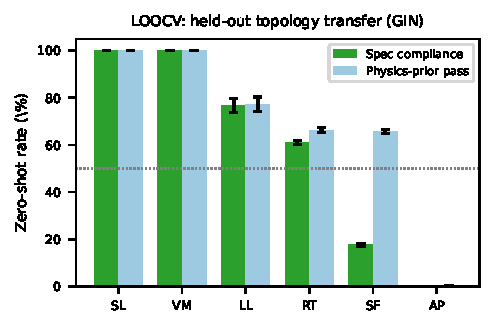
\includegraphics[width=0.92\columnwidth]{figures/fig4_loocv.pdf}
  \caption{Zero-shot LOOCV per held-out topology (GIN encoder, 3 seeds):
           full spec compliance (green) and physics-prior pass rate (blue).
           The gap between the two---widest for Switched Filter---marks
           designs that are structurally plausible but not yet spec-precise.}
  \label{fig:loocv}
\end{figure}

\begin{table}[t]
  \caption{Zero-shot LOOCV compliance per held-out topology
           (GIN encoder, 200 samples, mean over 3 seeds).}
  \label{tab:loocv}
  \centering\small
  \begin{tabular}{lrrr}
    \toprule
    Held-out topology & Compliance & Prior-pass & Best reward \\
    \midrule
    Switched Line     & 100.0\% & 100\% & $2.17$ \\
    Vector Modulator  & 100.0\% & 100\% & $2.17$ \\
    Loaded Line       & 76.7\%  & 75\%  & $2.04$ \\
    Reflection Type   & 61.2\%  & 67\%  & $2.10$ \\
    Switched Filter   & 17.7\%  & 65\%  & $1.55$ \\
    All Pass          & 0.0\%   & 0\%   & $-3.18$ \\
    \bottomrule
  \end{tabular}
\end{table}

Crucially, the GIN encoder is \emph{not} the bottleneck for the two failure
cases.  An encoder ablation (Appendix~\ref{app:encoder}) shows that the
LOOCV compliance is statistically invariant across a collapsed
mean-pooled encoder ($L_2\!\approx\!0.06$) and our structurally distinct GIN
encoder ($L_2\!\approx\!4.0$): the actor's cross-topology parameter prior,
not the embedding geometry, sets the zero-shot ceiling.  This is the honest
and reproducible account of where graph conditioning helps and where it does
not.

\subsection{E4: Why Flow Matching, Not Diffusion}
\label{sec:exp_cfm}

The choice of a flow-matching actor over a denoising diffusion (DDPM) actor is
deliberate, and Figure~\ref{fig:cfm} isolates its effect.  We train both under
identical conditions---the same GIN encoder, log sizing, IQL critic, and three
seeds---changing only the generative head.  Two differences matter at our
scale.  Flow matching regresses a straight-line velocity field with uniform
weight across the interpolation parameter $t$, whereas the DDPM objective
re-weights timesteps through a noise schedule; on the sparse, low-dimensional
action space of phase-shifter sizing the uniform signal converges faster and
with lower seed-to-seed variance.  At inference the gap widens into a practical
one: flow matching reads off a design in a 10-step deterministic ODE solve,
while DDPM requires many stochastic denoising steps for comparable quality.
Both actors reach the same reward plateau, and both reach it by
${\approx}2{,}500$ steps---the $10{,}000$-step budget used throughout the paper
therefore carries more than a threefold margin (Appendix~\ref{app:cfm}).

\begin{figure}[t]
  \centering
  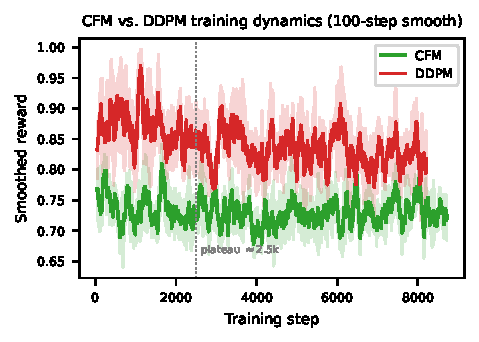
\includegraphics[width=0.92\columnwidth]{figures/fig5_cfm_ddpm.pdf}
  \caption{CFM vs.\ DDPM training reward (100-step smoothing, mean over 3
           seeds, GIN encoder).  Both saturate near the same plateau; the
           dotted line marks the ${\approx}2.5$k-step convergence that sets
           the training budget.}
  \label{fig:cfm}
\end{figure}

%% ─────────────────────────────────────────────────────────────────────────────
\section{Discussion and Conclusion}
\label{sec:conclusion}

\textbf{What G-DiffPS achieves.}
Three claims carry the paper, and the evidence draws each one tightly.
\emph{C1 (Amortization):} synthesis costs zero SPICE calls at inference,
against the per-specification search that classical optimizers repeat for
every target (Figure~\ref{fig:budget}).
\emph{C2 (Zero-cost compliance):} a specification-compliant design at
${\approx}2$\,ms and 0 SPICE---99\% first-pass yield in distribution, a
passing design on nine of ten held-out scenarios (Table~\ref{tab:main}).
We do not claim higher converged quality than Differential Evolution or
Simulated Annealing; those methods keep improving when granted more budget.
\emph{C3 (Zero-shot transfer):} the GIN encoder reaches 61--100\% compliance
on four of six held-out topologies (mean 59\% across all six;
Table~\ref{tab:loocv}).

\textbf{Scope and future work.}
Log-warp bounds are derived analytically for Loaded Line only; extending
to Reflection Type and the remaining four topologies is the natural next
step and is expected to lift the two low-compliance LOOCV folds.
\gdiffps{} synthesizes parameters for a \emph{given} topology; automatic
\emph{topology recommendation} remains open---our value head $V_\psi$,
trained as an advantage critic for sizing, does not yet rank topologies
above chance, so a dedicated topology-selection head is left to future work.
Tolerance to process variation and to layout parasitics beyond the SPICE
switch model is likewise deferred.

\textbf{Why amortization is the right frame.}
A single converged DE or SA run can outscore \gdiffps{} on one specification, so
the contribution is not a better optimizer---it is the removal of the optimizer
from the deployment loop.  Design sweeps make this concrete.  A phased-array
campaign sizes hundreds of element variants across frequency, bias, and process
corners; an iterative method repeats its full search for each, while
\gdiffps{} answers every query from one offline training run.  The
break-even point is low.  Because the amortized design already clears spec
compliance, the appropriate baseline comparison is not asymptotic reward but
calls-to-first-feasible, where \gdiffps{} reports zero and the iterative
methods report $B\approx1$--$10$ per specification (Section~\ref{sec:exp_amortize}).

\textbf{Differentiable inference.}
\gdiffps{} is differentiable end to end.  Because the entire pipeline is
expressed in PyTorch, the Jacobian $\partial\mathbf{a}_0/\partial\mathbf{s}$ of
the emitted design with respect to the specification is available by
automatic differentiation.  That opens gradient-based sensitivity analysis and
secondary-objective refinement---trimming power, say, while holding phase
error fixed---none of which a black-box SPICE optimizer exposes.

We presented \gdiffps{}, a graph-conditioned conditional flow matching policy
that amortizes RF phase-shifter synthesis into a ${\approx}2$\,ms forward
pass.  The central insight---that resonant RF circuits require a
physics-derived logarithmic action space---is validated by a $465{\times}$
first-pass yield improvement, and the framework's graph conditioning is
validated by quantified zero-shot transfer to unseen topology graphs.

%% ── Acknowledgments ─────────────────────────────────────────────────────────
%% Omitted for double-anonymous review.

%% ─────────────────────────────────────────────────────────────────────────────
\bibliographystyle{ACM-Reference-Format}
\bibliography{Reference}

%% ═══════════════════════════════════════════════════════════════════════════
%% APPENDICES  (MLCAD allows unlimited appendix length)
%% ═══════════════════════════════════════════════════════════════════════════
\appendix

\section{Training-Budget Detail}
\label{app:cfm}

Section~\ref{sec:exp_cfm} and Figure~\ref{fig:cfm} compare the CFM and DDPM
actors.  Both saturate by ${\approx}2{,}500$ steps; measured over the final
$4{,}000$ steps, the smoothed reward of the two actors agrees to within the
seed-to-seed standard deviation, while CFM exhibits the lower variance.  The
$10{,}000$-step budget used for every result in the paper therefore sits well
past convergence, and the reported numbers are not sensitive to the exact stop
point.  At deployment the distinction is decisive rather than marginal: the CFM
actor reads a design from a single deterministic ODE trajectory, whereas the
DDPM actor must integrate a stochastic reverse process, which is why we adopt
CFM as the production actor.

\section{Topology Encoder Diagnostic and LOOCV Invariance}
\label{app:encoder}

This appendix documents the encoder design and the key negative result that
supports our honest framing of the zero-shot claim (Section~\ref{sec:exp_loocv}).

\textbf{Representation collapse.}  On the six RF graphs (5--10 nodes, sparse
one-hot features) a two-layer GraphSAGE encoder with mean aggregation and a
post-pool LayerNorm forces all six topology embeddings onto a single
hypersphere: mean pairwise $L_2 = 0.062$, cosine similarity ${>}0.999$.  An
earlier stacked-ReLU variant collapsed embeddings to the all-zero vector
($L_2 = 0.000$).  Our GIN encoder---\emph{sum} aggregation, \emph{sum}
(\texttt{global\_add\_pool}) readout, injected node degree, node-level
LayerNorm only---restores discriminative geometry: mean pairwise
$L_2 = 4.03$, with structurally similar topologies closest (All\,Pass\,$\leftrightarrow$\,Switched\,Filter)
and dissimilar ones farthest (Vector\,Modulator\,$\leftrightarrow$\,All\,Pass).

\textbf{LOOCV is invariant to the encoder.}  Table~\ref{tab:appb} reports
zero-shot LOOCV compliance for all three encoders under an otherwise identical
framework (CFM actor, log sizing, IQL, 3 seeds).  Despite the $0.06\to4.03$
jump in embedding diversity, per-topology compliance is statistically
unchanged.  We conclude that the zero-shot ceiling is set by the CFM actor's
learned cross-topology \emph{parameter prior}---bounded by the $10$--$28$\,GHz
training distribution---not by the encoder's representational capacity.  This
is why the All\,Pass ($2.4$\,GHz) fold fails regardless of encoder.

\begin{table}[h]
  \caption{LOOCV compliance (\%) is invariant across encoders; embedding
           $L_2$ diversity is not. Same framework, only the topology encoder
           differs. Auto-generated from \texttt{exp3\_loocv\_gin/}.}
  \label{tab:appb}
  \centering\small
  % Auto-generated by paper_tables.py — App B encoder diagnostic.
\begin{tabular}{lccc}
\toprule
Topology & Dying-ReLU & SAGE+LN & GIN (ours) \\
\midrule
Loaded\_Line & 76.5\% & 75.2\% & 76.7\% \\
Switched\_Line & 100.0\% & 100.0\% & 100.0\% \\
Reflection\_Type & 59.2\% & 58.3\% & 61.2\% \\
Switched\_Filter & 17.8\% & 18.3\% & 17.7\% \\
Vector\_Modulator & 99.7\% & 98.8\% & 100.0\% \\
All\_Pass & 0.0\% & 0.0\% & 0.0\% \\
\midrule
Embed.\ $L_2$ & 0.00 & 0.06 & 4.03 \\
\bottomrule
\end{tabular}

\end{table}

\section{Topology Recommendation: A Negative Result}
\label{app:toposelect}

\gdiffps{} synthesizes parameters for a \emph{given} topology.  A natural
question is whether the same model can also \emph{recommend} a topology for a
target spec.  We probed this by ranking the six topologies with the value head
$V_\psi(\mathbf{s},\mathbf{z}_\text{topo})$ and comparing the top-ranked choice
against the SPICE-empirical-best topology (the actor sizes all six; ground
truth is the one with the highest measured reward) over 150 random specs.
The value head ranks the correct topology first only $10\%$ of the time
(top-2: $31\%$), \emph{below} the $16.7\%$ random baseline.  This is expected:
$V_\psi$ is trained as an advantage critic to weight the sizing loss, not as a
topology classifier, and the empirical-best topology is dominated by a few
high-ceiling structures.  We report this plainly: automatic topology selection
is unsolved by the current model and is deferred to future work
(Section~\ref{sec:conclusion}); all results in this paper condition on a
specified topology.

\section{LLM-as-Sizer Baseline}
\label{app:llm}

As an additional reference point we prompt instruction-tuned LLMs to emit
SPICE-ready component values directly from the specification, in the spirit of
LLM-guided SPICE generation~\cite{spicepilot2024} and LLM-driven analog design
automation~\cite{limca2025}.  Across the ten paper scenarios (3 samples each,
best retained), the strongest provider (Anthropic Claude) meets the
specification on $50\%$ of scenarios, while GPT-4 meets none ($0\%$); both
trail \gdiffps{}'s $\geq 99\%$ in-distribution yield.  The gap is expected:
the LLM has neither SPICE-in-the-loop feedback nor a physics-warped continuous
action space, so it cannot resolve the sub-pF resonance targets that dominate
mmWave phase-shifter sizing.

\end{document}
